\section{Tổng Quan và Mục Tiêu Bài Thực Hành 1}

\subsection{Giới thiệu}
Bài thực hành 1 làm quen với nền tảng điện toán đám mây vạn vật kết nối \textbf{CoreIOT} (phát triển trên nền tảng mã nguồn mở ThingsBoard). Hệ thống cung cấp hạ tầng quản lý vòng đời thiết bị, bảo mật danh tính qua mã thông báo bí mật (Access Token), thu thập dữ liệu viễn trắc (Telemetry) và cơ chế điều khiển hai chiều thời gian thực thông qua lời gọi thủ tục từ xa (Remote Procedure Call - RPC) qua giao thức MQTT.

\subsection{Mục tiêu bài thực hành}
\begin{itemize}
    \item Đăng nhập và quản trị nền tảng CoreIOT với vai trò Tenant Administrator.
    \item Khởi tạo thiết bị, cấu hình Access Token bảo mật độc quyền và tổ chức thiết bị vào các nhóm (Entity Groups).
    \item Viết và chạy chương trình Python sử dụng thư viện MQTT (\texttt{paho-mqtt 2.x}) để gửi dữ liệu chuỗi thời gian gồm nhiệt độ, độ ẩm và cường độ ánh sáng lên máy chủ CoreIOT theo chu kỳ 3 giây.
    \item Thiết kế giao diện Dashboard giám sát thời gian thực với các thẻ chỉ thị số (Value Cards) và biểu đồ chuỗi thời gian (Time series chart).
    \item Hiện thực cơ chế RPC hai chiều (Two-way RPC) để điều khiển bật/tắt thiết bị chấp hành (LED, Máy bơm và Quạt làm mát) từ Dashboard và phản hồi trạng thái về máy chủ.
    \item Cấu hình phân quyền kế thừa thực thể và chia sẻ Dashboard công khai (Public Dashboard) xem được trên chế độ ẩn danh không cần đăng nhập.
\end{itemize}

\subsection{Bảng thông số cấu hình thực nghiệm}
\begin{table}[H]
\centering
\caption{Bảng cấu hình thông số kỹ thuật thực nghiệm trên CoreIOT}
\label{tab:iot_lab1_config}
\begin{tabularx}{\textwidth}{|p{4.5cm}|p{4.8cm}|X|}
\hline
\textbf{Thuộc tính} & \textbf{Giá trị cấu hình} & \textbf{Mục đích / Ghi chú} \\
\hline
Họ và tên sinh viên & Phạm Công Võ & Sinh viên thực hiện \\
Mã số sinh viên & \texttt{2313946} & Định danh sinh viên \\
Tên thiết bị (Device Name) & \texttt{Lab1\_2313946} & Định danh thiết bị trên CoreIOT \\
Device Profile & \texttt{default} & Luồng xử lý quy tắc mặc định \\
Credentials Type & \texttt{Access token} & Xác thực MQTT qua Username ($\ge 12$ ký tự) \\
Nhóm thiết bị (Device Group) & \texttt{LAB1\_2313946\_group} & Gom nhóm quản lý và chia sẻ công khai \\
Tên Dashboard & \texttt{LAB1\_2313946 Dashboard} & Bảng điều khiển trực quan hóa dữ liệu \\
Server Broker & \texttt{app.coreiot.io} & Máy chủ đám mây CoreIOT (Port 1883) \\
\hline
\end{tabularx}
\end{table}

\newpage
\section{Nội Dung Chi Tiết Các Bài Tập Thực Hành}

% =============================================================================
% BÀI 1
% =============================================================================
\subsection{Bài 1: Tạo thiết bị, thông tin xác thực và nhóm thiết bị (1.5 Điểm)}

\begin{tcolorbox}[
    enhanced, colback=black!2, colframe=black!60, boxrule=1pt, arc=2.5mm, drop shadow,
    attach boxed title to top left={xshift=4mm, yshift=-3mm},
    boxed title style={enhanced, colback=black!85, colframe=black!85, boxrule=1pt, arc=2.5mm, drop shadow, left=6pt, right=6pt, top=2pt, bottom=2pt},
    title=\textcolor{white}{\large\textbf{Yêu cầu đề bài (Trích phiếu bài tập)}}
]
\bfseries
\vspace{0.2cm}
\begin{itemize}
    \item Tạo một thiết bị tên \texttt{Lab1\_2313946} với Device Profile \texttt{default}.
    \item Mở Manage credentials và đặt một Access Token tùy chỉnh do bạn chọn (ít nhất 12 ký tự). Lưu lại.
    \item Tạo một nhóm thiết bị tên \texttt{LAB1\_2313946\_group} và thêm thiết bị của bạn vào nhóm.
    \item Chụp 3 ảnh minh chứng: Trang Details thiết bị, Hộp thoại Credentials (làm mờ token), và Danh sách nhóm.
    \item Trả lời Câu hỏi 1.
\end{itemize}
\end{tcolorbox}

\vspace{0.3cm}
\subsubsection{Hình ảnh minh chứng thực nghiệm}

\begin{figure}[H]
    \centering
    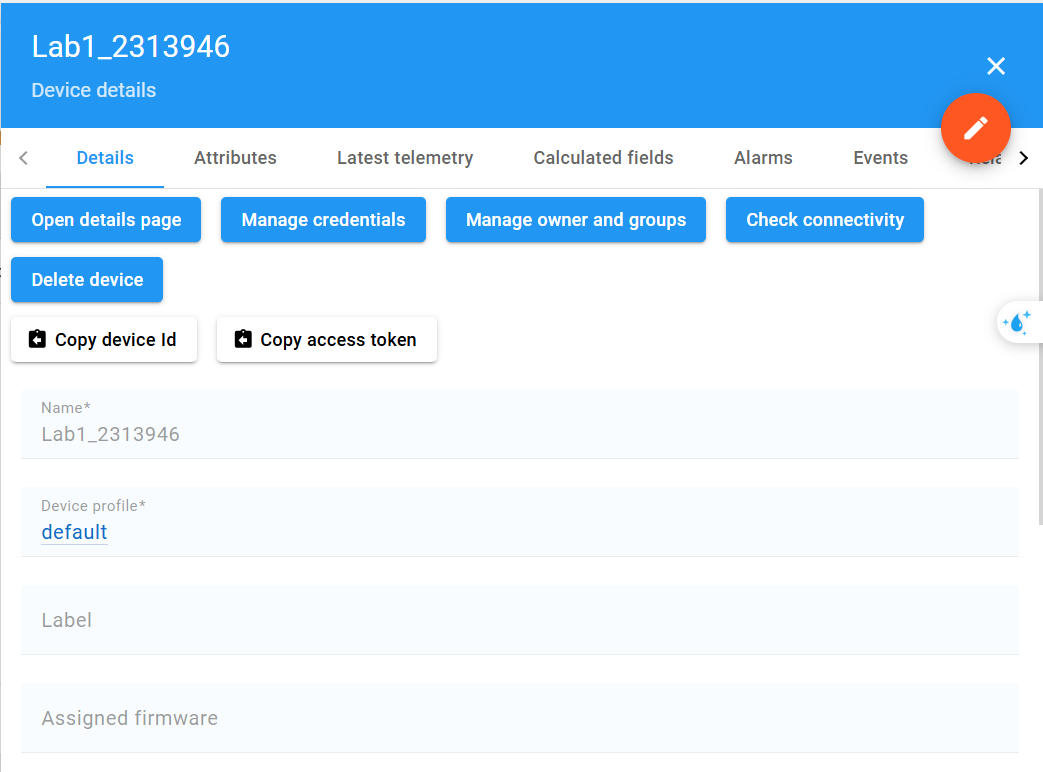
\includegraphics[width=0.9\textwidth]{image/anh1_1.png}
    \caption{Trang chi tiết thiết bị (Tab Details) hiển thị tên thiết bị \texttt{Lab1\_2313946}}
    \label{fig:anh1_1}
\end{figure}

\begin{figure}[H]
    \centering
    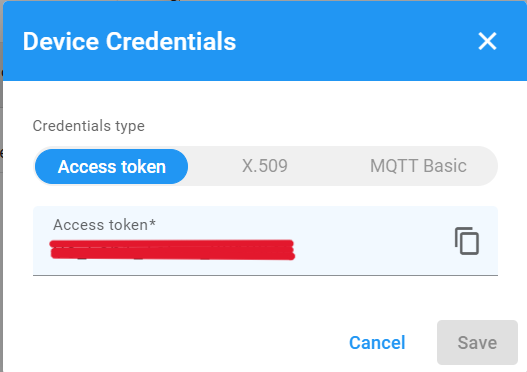
\includegraphics[width=0.57\textwidth]{image/anh1_2.png}
    \caption{Hộp thoại Device Credentials chọn Access token (giá trị token đã được che bảo mật)}
    \label{fig:anh1_2}
\end{figure}

\begin{figure}[H]
    \centering
    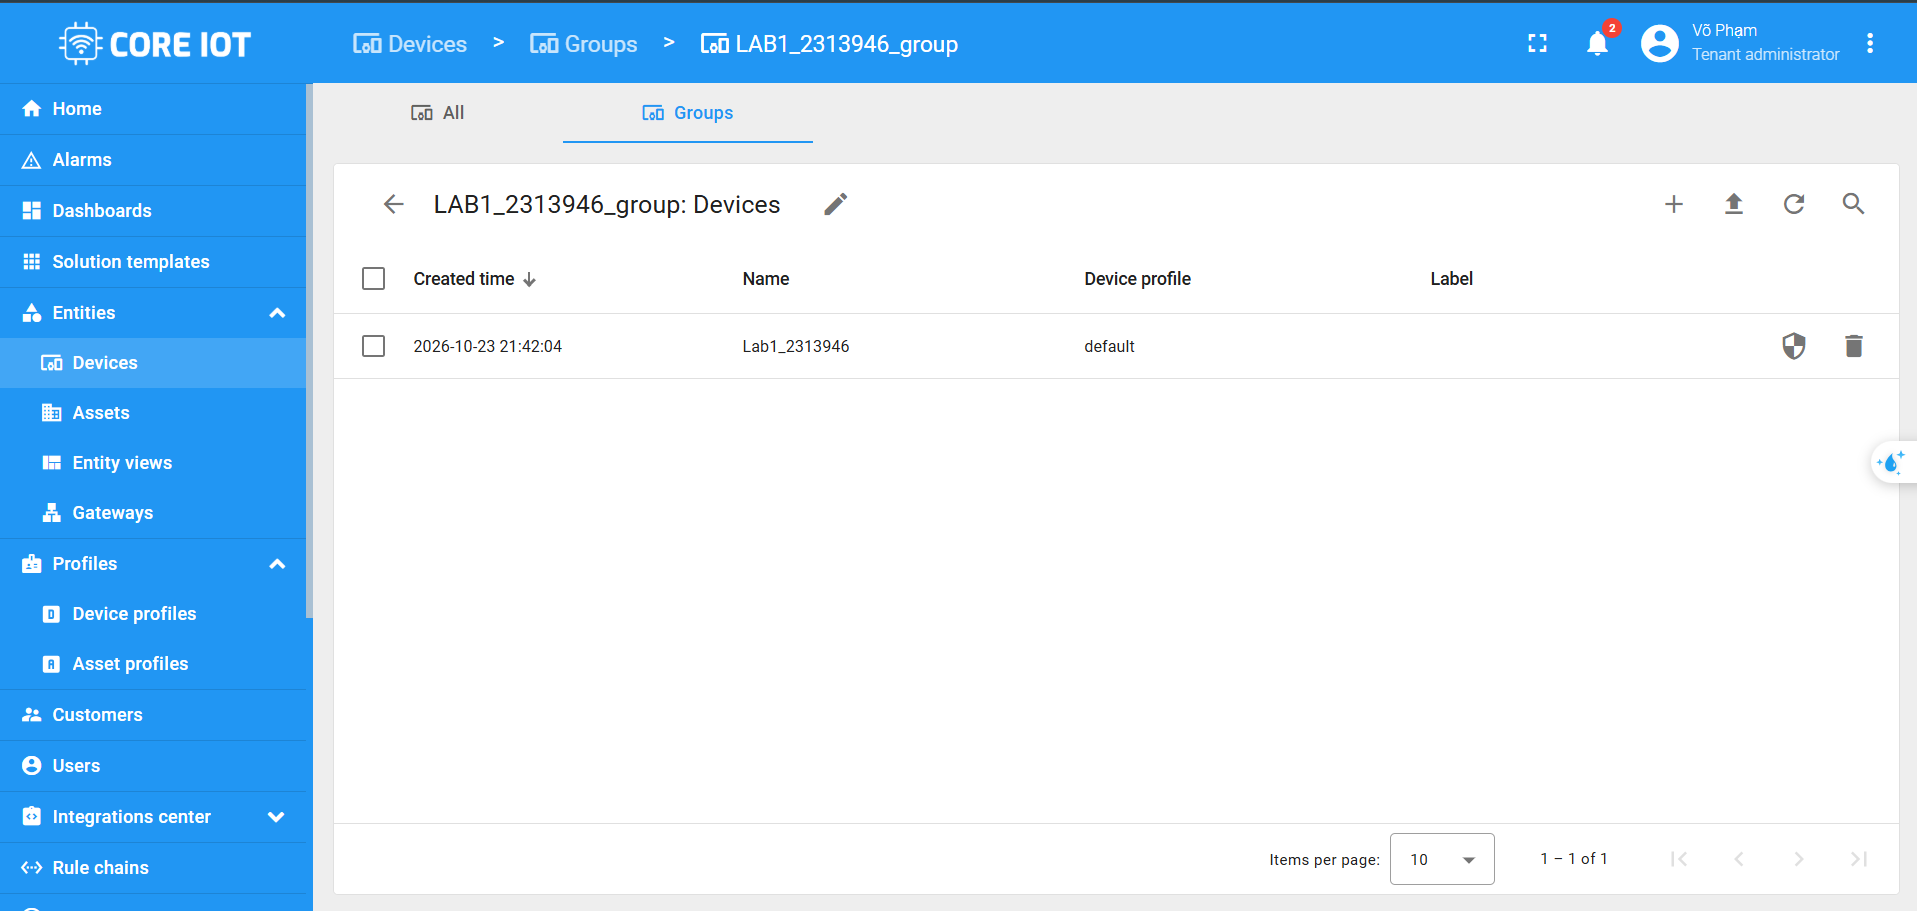
\includegraphics[width=0.85\textwidth]{image/anh1_3.png}
    \caption{Nhóm thiết bị \texttt{LAB1\_2313946\_group} hiển thị thiết bị bên trong và quyền quản trị viên}
    \label{fig:anh1_3}
\end{figure}

\begin{tcolorbox}[colback=blue!5,colframe=blue!75!black,title=\textbf{Câu hỏi 1: Sự khác nhau giữa hai loại thông tin xác thực Access token và MQTT Basic là gì? Vì sao phải giữ bí mật token?}]
\textbf{Trả lời:}
\begin{itemize}
    \item \textbf{Sự khác nhau:} \textit{Access token} sử dụng một chuỗi ký tự bí mật duy nhất được truyền trong trường \texttt{Username} của bản tin kết nối MQTT (bỏ trống trường Password), giúp cơ chế bắt tay kết nối cực kỳ gọn nhẹ, tối ưu cho các vi điều khiển và thiết bị IoT bị giới hạn tài nguyên tính toán. Trong khi đó, \textit{MQTT Basic} yêu cầu cấu hình đầy đủ bộ ba thông tin gồm: \texttt{Client ID}, \texttt{User Name} và \texttt{Password}.
    \item \textbf{Vì sao phải giữ bí mật token:} Access token đóng vai trò là "chìa khóa định danh độc quyền" của thiết bị trên hệ thống CoreIOT. Nếu token bị rò rỉ, kẻ xấu từ bất kỳ đâu trên Internet đều có thể giả mạo thiết bị để bơm dữ liệu giả mạo (Data Poisoning) làm sai lệch kết quả giám sát, hoặc nguy hiểm hơn là gửi các lệnh điều khiển trái phép can thiệp vào hoạt động của thiết bị phần cứng thực tế.
\end{itemize}
\end{tcolorbox}

\newpage
% =============================================================================
% BÀI 2
% =============================================================================
\subsection{Bài 2: Gửi telemetry từ Python kèm cảm biến ánh sáng (2.0 Điểm)}

\begin{tcolorbox}[
    enhanced, colback=black!2, colframe=black!60, boxrule=1pt, arc=2.5mm, drop shadow,
    attach boxed title to top left={xshift=4mm, yshift=-3mm},
    boxed title style={enhanced, colback=black!85, colframe=black!85, boxrule=1pt, arc=2.5mm, drop shadow, left=6pt, right=6pt, top=2pt, bottom=2pt},
    title=\textcolor{white}{\large\textbf{Yêu cầu đề bài (Trích phiếu bài tập)}}
]
\bfseries
\vspace{0.2cm}
\begin{itemize}
    \item Bắt đầu từ script \texttt{lab1\_device.py} và đặt Access Token bí mật của bạn.
    \item Thêm khóa telemetry thứ ba tên \texttt{light} với giá trị số nguyên ngẫu nhiên từ 0 đến 1000 (\texttt{random.randint(0, 1000)}).
    \item Đổi chu kỳ gửi dữ liệu từ 5 giây thành 3 giây (\texttt{time.sleep(3)}).
    \item Chạy script ít nhất một phút và kiểm tra dữ liệu trên CoreIOT.
    \item Chụp ảnh màn hình Terminal và tab Latest telemetry của thiết bị.
    \item Trả lời Câu hỏi 2.
\end{itemize}
\end{tcolorbox}

\vspace{0.3cm}
\subsubsection{Mã nguồn Python gửi Telemetry (Mã 2.1)}
\begin{lstlisting}[language=Python, caption={Vòng lặp gửi dữ liệu viễn trắc định kỳ mỗi 3 giây trong lab1\_device.py}]
try:
    while True:
        # Thu thap cac thong so cam bien mo phong
        temp = round(random.uniform(25.0, 35.0), 1)
        humi = round(random.uniform(50.0, 85.0), 1)
        light = random.randint(0, 1000)

        # Dong goi payload JSON gom du 3 dai luong
        payload = {
            "temperature": temp,
            "humidity": humi,
            "light": light
        }
        
        # Gui du lieu len topic Telemetry chuan cua CoreIOT
        client.publish("v1/devices/me/telemetry", json.dumps(payload), qos=1)
        print(f"Sent: {payload}")
        
        # Yeu cau de bai: Chu ky truyen gui du lieu la 3 giay
        time.sleep(3)
except KeyboardInterrupt:
    print("\nDang ngat ket noi...")
\end{lstlisting}

\subsubsection{Hình ảnh minh chứng thực nghiệm}

\begin{figure}[H]
    \centering
    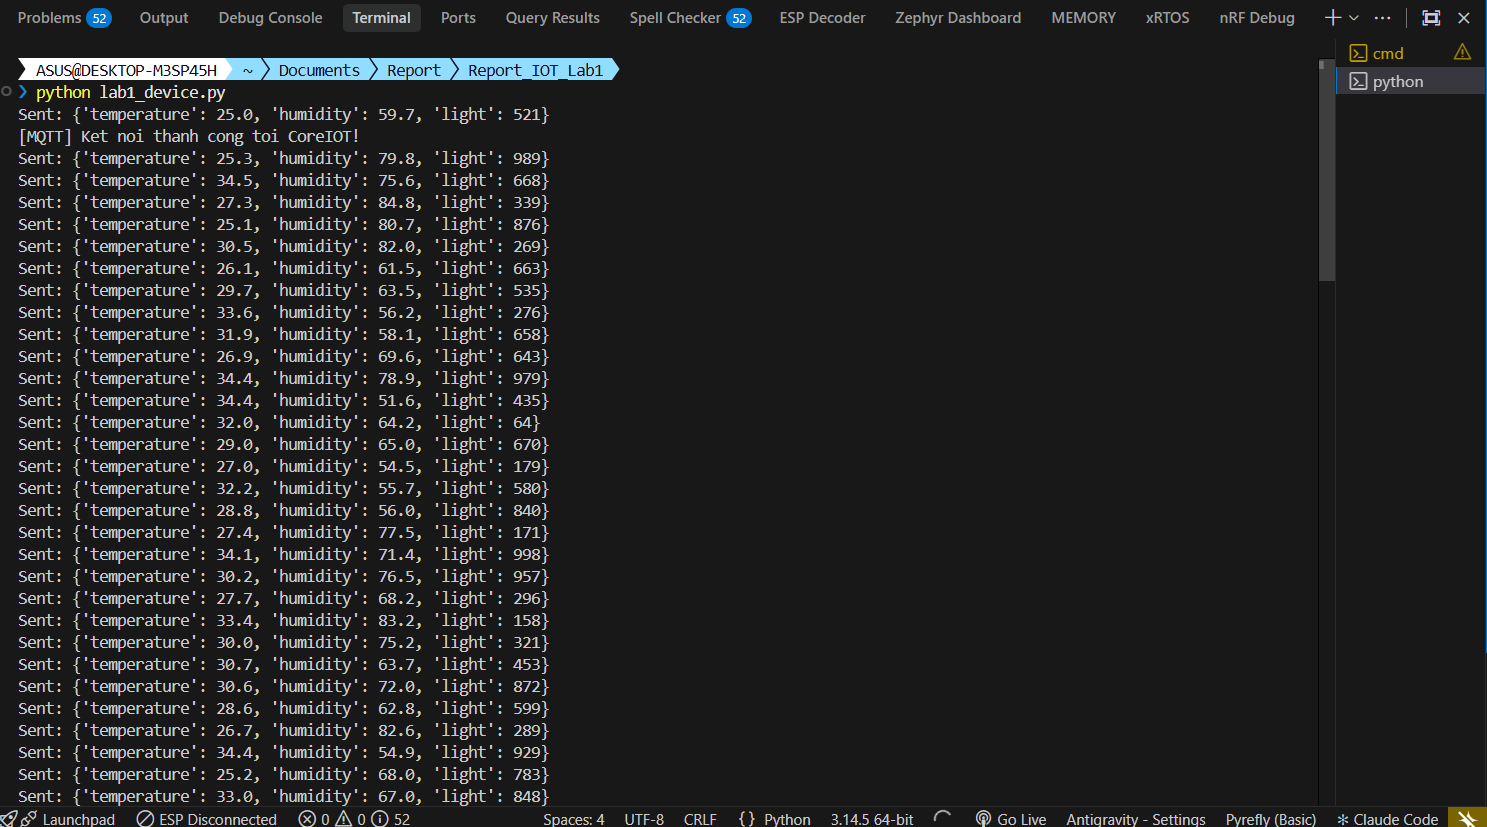
\includegraphics[width=0.88\textwidth]{image/anh2_1.png}
    \caption{Terminal hiển thị kết nối thành công và các dòng Sent chứa cả 3 khóa bao gồm \texttt{light}}
    \label{fig:anh2_1}
\end{figure}

\begin{figure}[H]
    \centering
    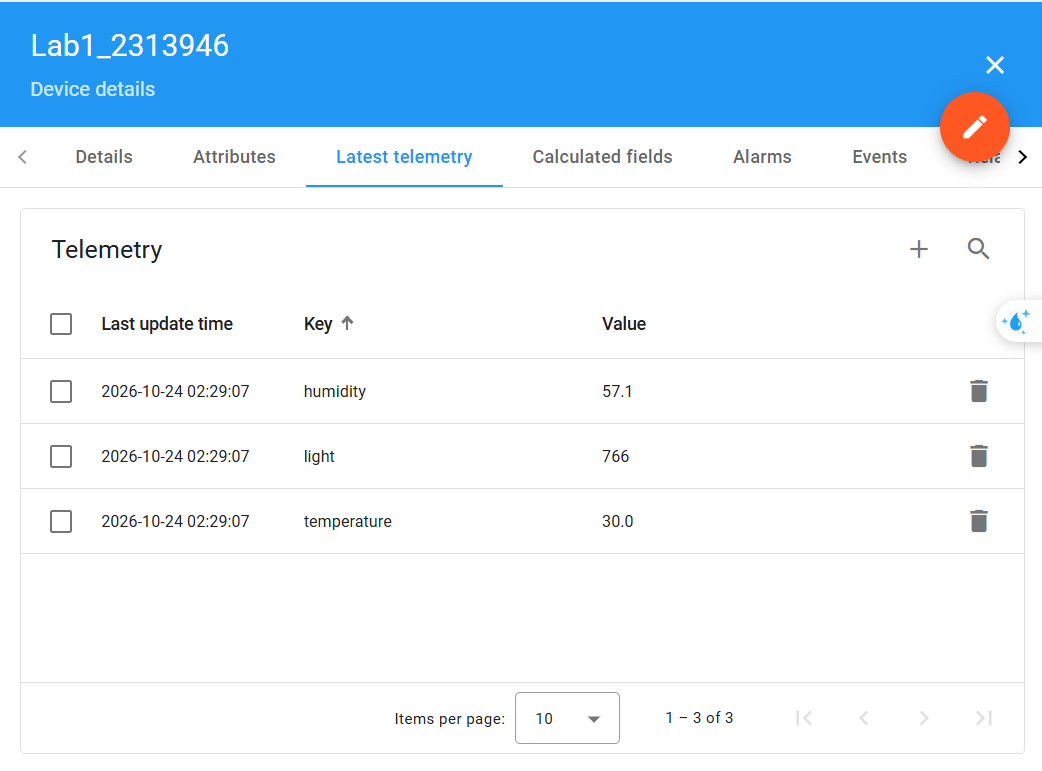
\includegraphics[width=0.85\textwidth]{image/anh2_2.png}
    \caption{Tab Latest telemetry của thiết bị \texttt{Lab1\_2313946} hiển thị đầy đủ 3 khóa dữ liệu}
    \label{fig:anh2_2}
\end{figure}

\subsubsection{Trả lời câu hỏi bài tập 2}
\begin{tcolorbox}[colback=blue!5,colframe=blue!75!black,title=\textbf{Câu hỏi 2: Script gửi telemetry lên MQTT topic nào, và một bản tin trông như thế nào (viết một ví dụ payload JSON)?}]
\textbf{Trả lời:}
\begin{itemize}
    \item \textbf{MQTT Topic:} Script gửi dữ liệu viễn trắc lên topic chuẩn theo quy ước ThingsBoard/CoreIOT:
    \begin{center}
        \texttt{v1/devices/me/telemetry}
    \end{center}
    Trong đó ký tự \texttt{"me"} đại diện cho chính thiết bị sở hữu Access Token đang được kết nối.
    \item \textbf{Ví dụ bản tin JSON Payload thực tế:}
\begin{lstlisting}[language=Python]
{"temperature": 28.5, "humidity": 68.2, "light": 650}
\end{lstlisting}
    Bản tin gồm 3 cặp khóa-giá trị: nhiệt độ đo theo độ C, độ ẩm tương đối tính theo \%, và cường độ ánh sáng đo theo đơn vị Lux.
\end{itemize}
\end{tcolorbox}

\newpage
% =============================================================================
% BÀI 3
% =============================================================================
\subsection{Bài 3: Xây dựng Dashboard giám sát (2.5 Điểm)}

\begin{tcolorbox}[
    enhanced, colback=black!2, colframe=black!60, boxrule=1pt, arc=2.5mm, drop shadow,
    attach boxed title to top left={xshift=4mm, yshift=-3mm},
    boxed title style={enhanced, colback=black!85, colframe=black!85, boxrule=1pt, arc=2.5mm, drop shadow, left=6pt, right=6pt, top=2pt, bottom=2pt},
    title=\textcolor{white}{\large\textbf{Yêu cầu đề bài (Trích phiếu bài tập)}}
]
\bfseries
\vspace{0.2cm}
\begin{itemize}
    \item Tạo một Dashboard mới tên \texttt{LAB1\_2313946 Dashboard}.
    \item Thêm ba widget Value card: Nhiệt độ ($^\circ$C), Độ ẩm (\%), và Ánh sáng (lx), cấu hình nhãn, đơn vị và biểu tượng phù hợp.
    \item Thêm một Widget Time series chart hiển thị đồng thời cả ba khóa dữ liệu dưới dạng các chuỗi (series) riêng biệt.
    \item Sắp xếp gọn gàng và lưu lại Dashboard.
    \item Trả lời Câu hỏi 3.
\end{itemize}
\end{tcolorbox}

\vspace{0.3cm}
\subsubsection{Hình ảnh minh chứng thực nghiệm}

\begin{figure}[H]
    \centering
    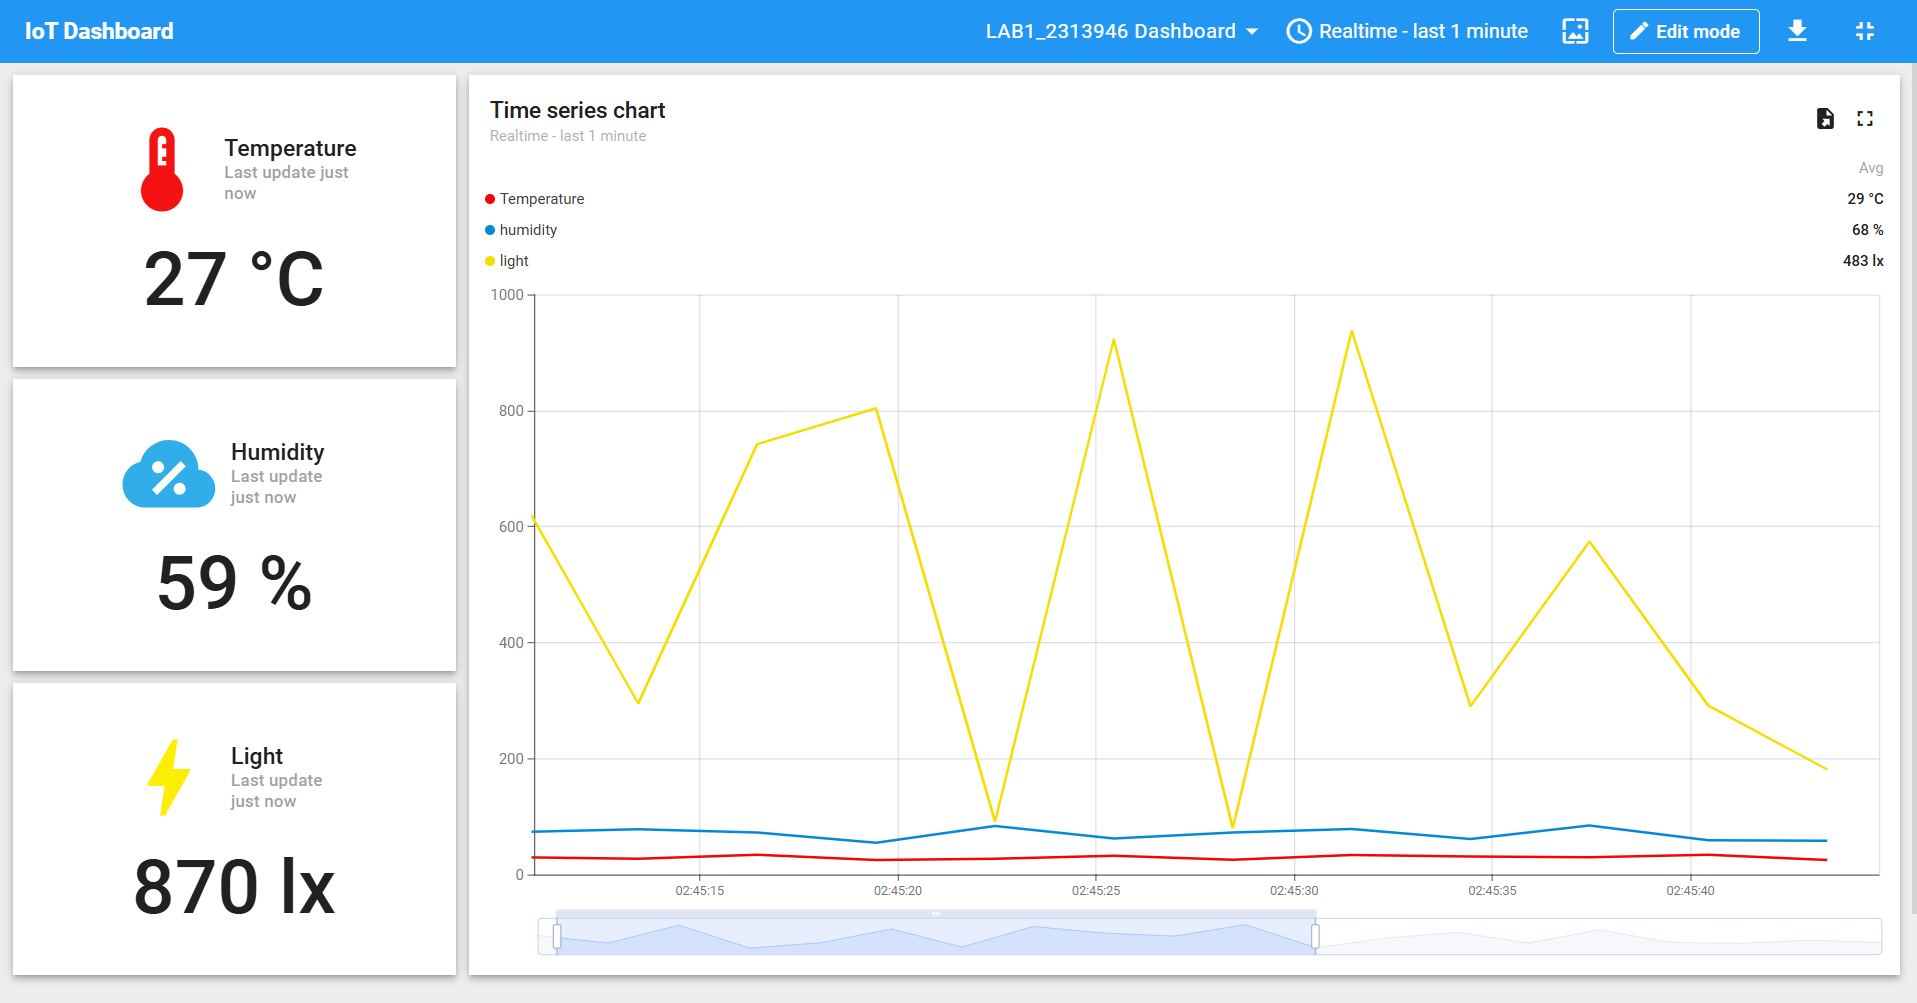
\includegraphics[width=\textwidth]{image/anh3_1.png}
    \caption{Toàn bộ giao diện \texttt{LAB1\_2313946 Dashboard} hiển thị trực quan 3 thẻ số và biểu đồ đường}
    \label{fig:anh3_1}
\end{figure}

\begin{figure}[H]
    \centering
    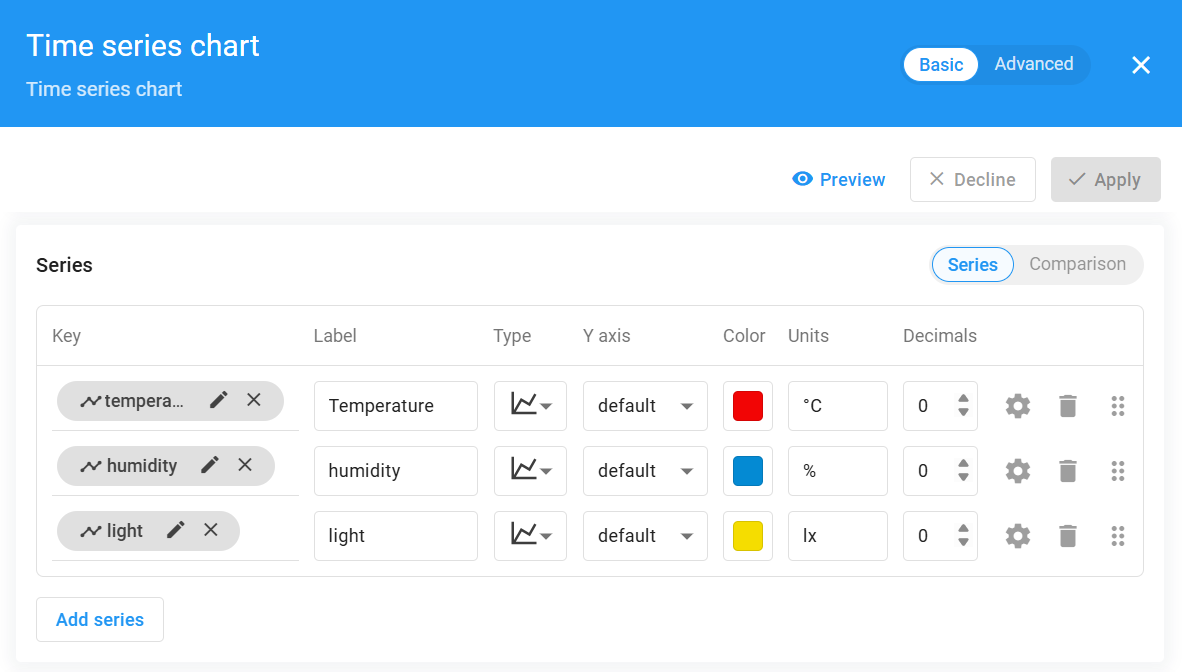
\includegraphics[width=\textwidth]{image/anh3_2.png}
    \caption{Cấu hình trình chỉnh sửa widget Time series chart hiển thị đủ 3 chuỗi dữ liệu (Series)}
    \label{fig:anh3_2}
\end{figure}

\subsubsection{Trả lời câu hỏi bài tập 3}
\begin{tcolorbox}[colback=blue!5,colframe=blue!75!black,title=\textbf{Câu hỏi 3: Khi bạn thêm Value card lần đầu, vì sao khóa light có thể không xuất hiện trong danh sách data key? Bạn khắc phục bằng cách nào?}]
\textbf{Trả lời:}
\begin{itemize}
    \item \textbf{Nguyên nhân:} Nền tảng CoreIOT chỉ tự động phát hiện, lập chỉ mục và gợi ý danh mục Data Key trong trình thiết kế widget sau khi máy chủ nhận được ít nhất một bản tin telemetry chứa khóa đó từ thiết bị gửi lên. Nếu script Python chưa chạy hoặc chưa gửi gói tin nào có trường \texttt{light}, máy chủ sẽ coi như khóa này chưa từng tồn tại trên thiết bị.
    \item \textbf{Cách khắc phục:}
    \begin{enumerate}
        \item Khởi động script Python chạy trước khoảng vài chu kỳ để gửi dữ liệu có chứa khóa \texttt{light} lên hệ thống, sau đó quay lại trang chỉnh sửa widget.
        \item Hoặc có thể tự nhập trực tiếp chuỗi ký tự \texttt{"light"} vào ô tìm kiếm Data Key trên giao diện Datasources rồi nhấn phím \textbf{Enter} để thiết lập thủ công.
    \end{enumerate}
\end{itemize}
\end{tcolorbox}

\newpage
% =============================================================================
% BÀI 4
% =============================================================================
\subsection{Bài 4: Điều khiển từ xa bằng RPC (2.5 Điểm)}

\begin{tcolorbox}[
    enhanced, colback=black!2, colframe=black!60, boxrule=1pt, arc=2.5mm, drop shadow,
    attach boxed title to top left={xshift=4mm, yshift=-3mm},
    boxed title style={enhanced, colback=black!85, colframe=black!85, boxrule=1pt, arc=2.5mm, drop shadow, left=6pt, right=6pt, top=2pt, bottom=2pt},
    title=\textcolor{white}{\large\textbf{Yêu cầu đề bài (Trích phiếu bài tập)}}
]
\bfseries
\vspace{0.2cm}
\begin{itemize}
    \item Thêm các widget Single Switch cho LED và Pump (Máy bơm) vào Dashboard.
    \item Thêm công tắc thứ ba cho Fan (Quạt) sử dụng các phương thức RPC \texttt{getStateFAN} và \texttt{setStateFAN}.
    \item Cập nhật script Python để lưu trữ trạng thái Quạt trong từ điển \texttt{state}, trả lời các yêu cầu \texttt{getState} và \texttt{setState}, in ra thông báo rõ ràng khi có thay đổi trạng thái (\texttt{-> ON} / \texttt{-> OFF}).
    \item Bật/tắt mỗi công tắc, tải lại Dashboard và kiểm tra tính nhất quán trạng thái.
    \item Trả lời Câu hỏi 4.
\end{itemize}
\end{tcolorbox}

\vspace{0.3cm}
\subsubsection{Mã nguồn Python xử lý RPC và phản hồi hai chiều (Mã 4.1)}
\begin{lstlisting}[language=Python]
state = {"LED": False, "PUMP": False, "FAN": False}

def on_message(client, userdata, msg):
    # Trich xuat request_id tu topic: v1/devices/me/rpc/request/{request_id}
    request_id = msg.topic.split("/")[-1]
    try:
        req = json.loads(msg.payload)
    except json.JSONDecodeError:
        print("[RPC] Payload JSON khong hop le:", msg.payload)
        return

    method = req.get("method", "")
    params = req.get("params")
    result = None

    # Xu ly getState: tra ve trang thai khi widget hoac Dashboard khoi tao
    if method.startswith("getState"):
        name = method[len("getState"):]
        result = state.get(name, False)

    # Xu ly setState: nhan lenh bat/tat tu Dashboard
    elif method.startswith("setState"):
        name = method[len("setState"):]
        if name in state:
            state[name] = bool(params)
            result = state[name]
            status_str = "ON" if result else "OFF"
            print(f"[DIEU KHIEN] {name} -> {status_str}")
            # Dong bo thuoc tinh len CoreIOT
            client.publish("v1/devices/me/attributes", 
                           json.dumps({name.lower() + "_state": result}))

    # Bat buoc phan hoi ve topic response de Widget xac nhan lenh thanh cong
    client.publish(f"v1/devices/me/rpc/response/{request_id}", 
                   json.dumps(result), qos=1)
\end{lstlisting}

\subsubsection{Hình ảnh minh chứng thực nghiệm}

\begin{figure}[H]
    \centering
    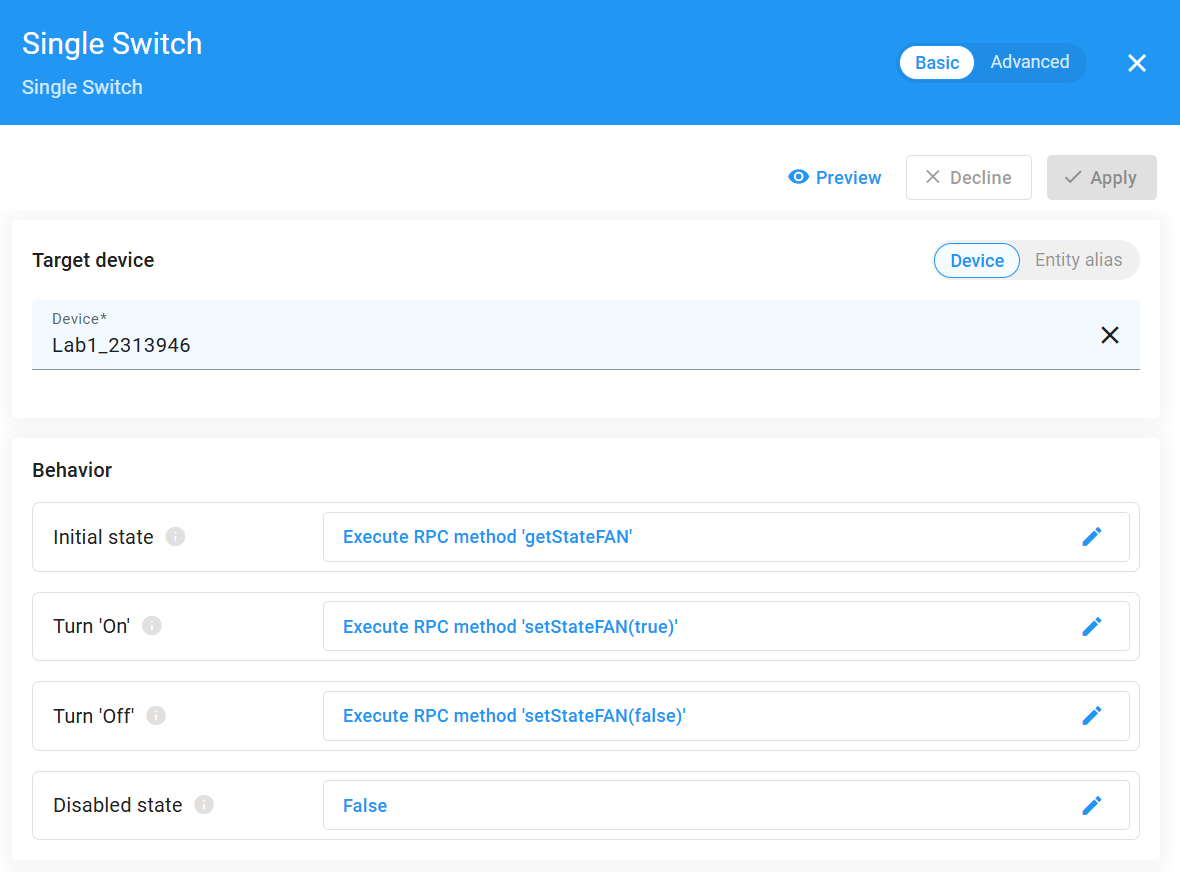
\includegraphics[width=0.94\textwidth]{image/anh4_1.png}
    \caption{Cấu hình tab Behavior của widget Quạt (Fan) với đầy đủ 3 phương thức RPC}
    \label{fig:anh4_1}
\end{figure}

\begin{figure}[H]
    \centering
    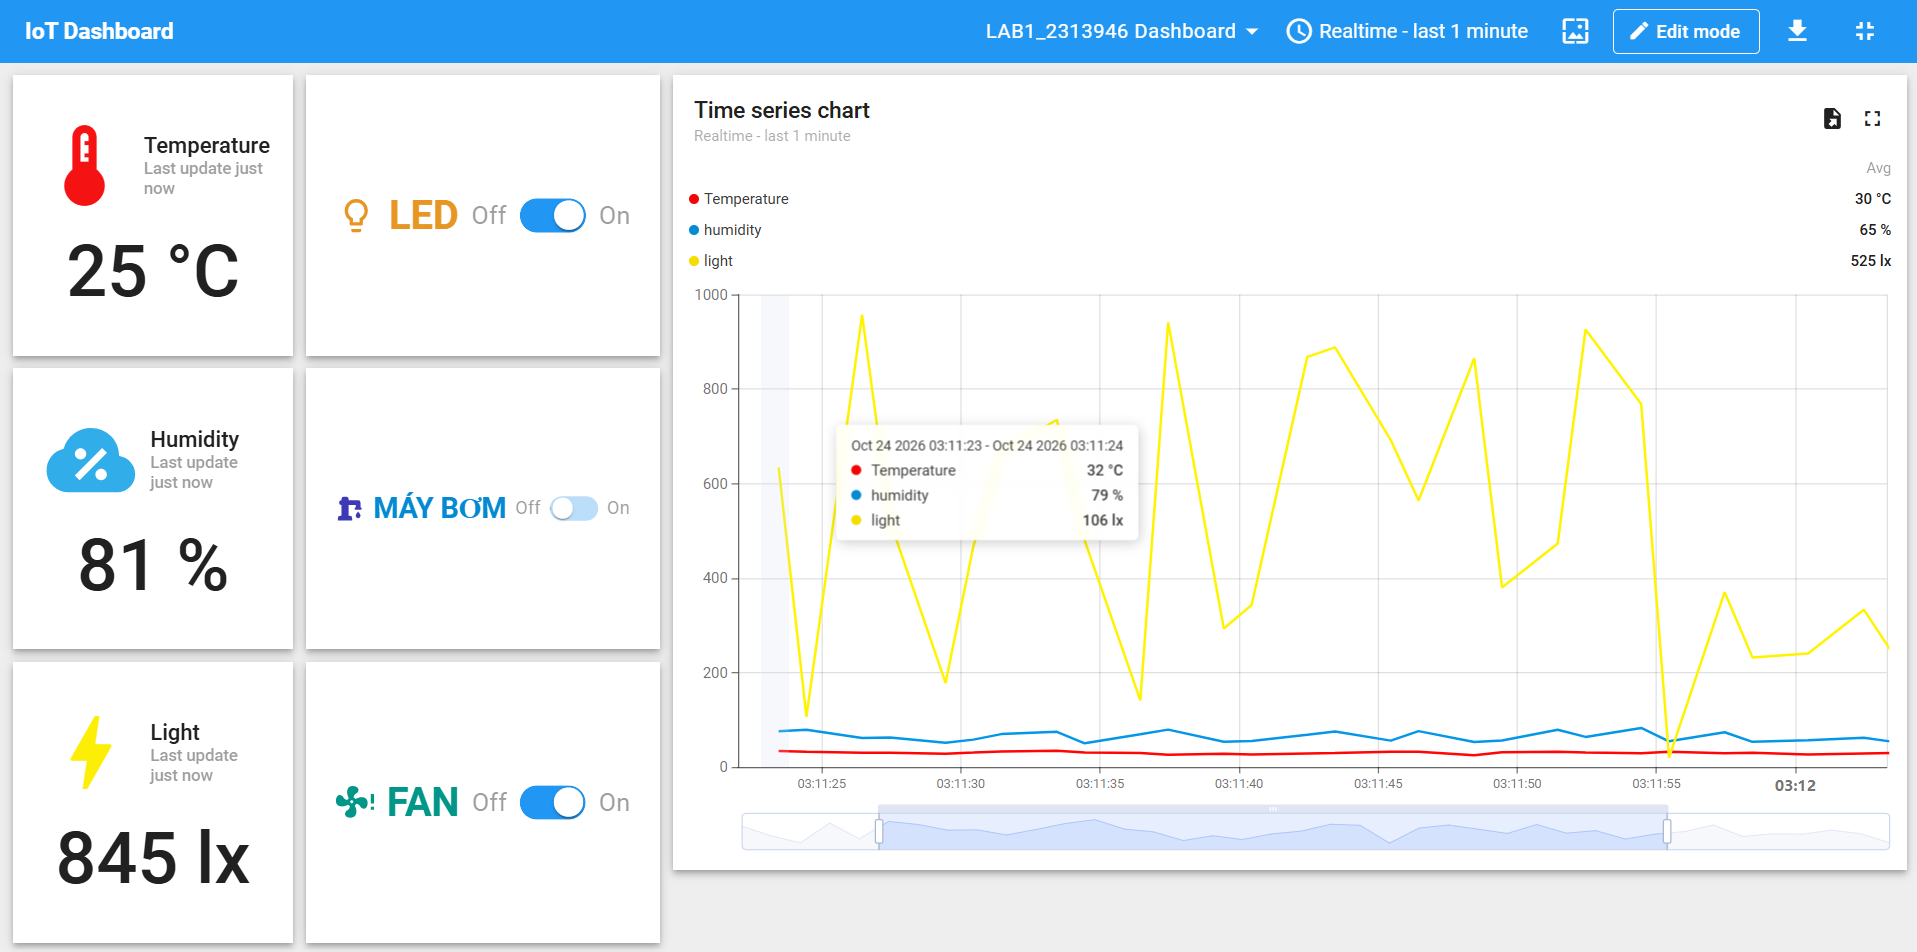
\includegraphics[width=\textwidth]{image/anh4_2.png}
    \caption{Dashboard hoàn chỉnh với 3 công tắc LED, MÁY BƠM, FAN sau khi đã điều khiển bật/tắt}
    \label{fig:anh4_2}
\end{figure}

\begin{figure}[H]
    \centering
    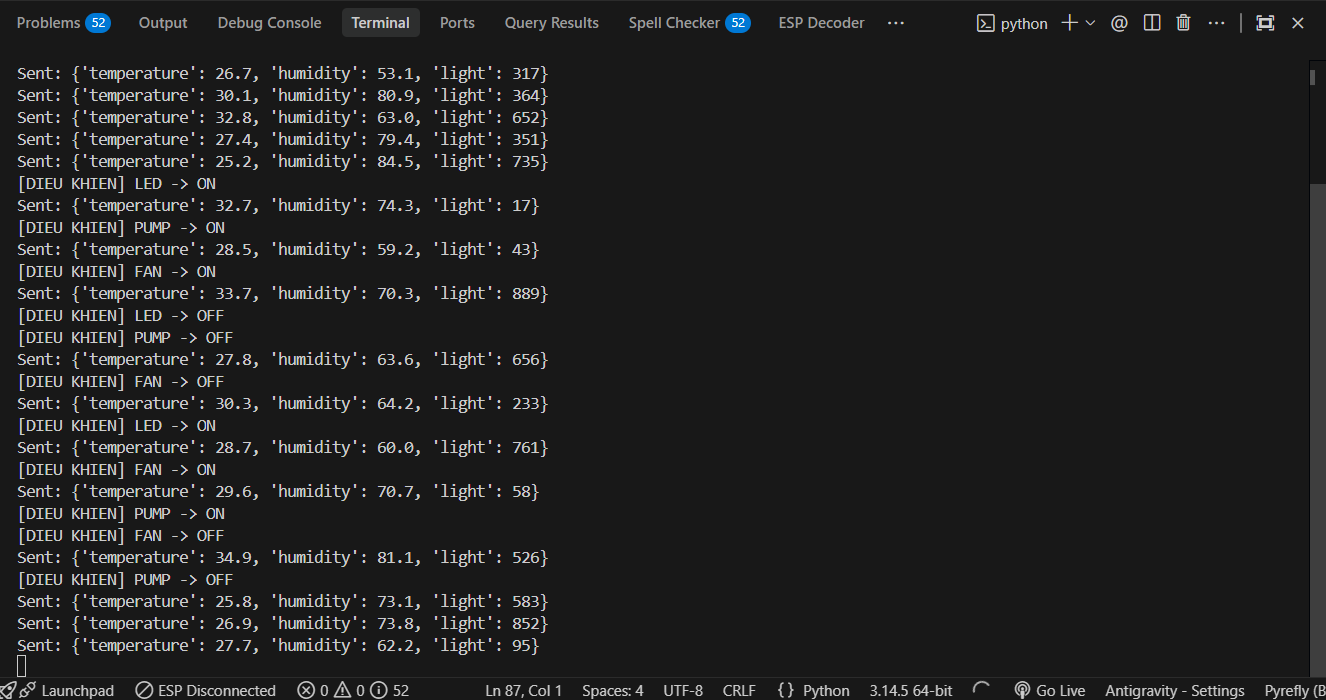
\includegraphics[width=\textwidth]{image/anh4_3.png}
    \caption{Terminal hiển thị log nhận lệnh RPC và in rõ ràng các thông báo trạng thái \texttt{-> ON} / \texttt{-> OFF}}
    \label{fig:anh4_3}
\end{figure}

\subsubsection{Trả lời câu hỏi bài tập 4}
\begin{tcolorbox}[colback=blue!5,colframe=blue!75!black,title=\textbf{Câu hỏi 4: Dừng script và bật/tắt một công tắc. Widget hiển thị gì, và vì sao? Vì sao thiết bị phải gửi phản hồi tới v1/devices/me/rpc/response/\{id\}?}]
\textbf{Trả lời:}
\begin{itemize}
    \item \textbf{Khi dừng script và gạt công tắc:} Widget công tắc sẽ chuyển sang biểu tượng quay vòng chờ đợi, sau vài giây sẽ báo lỗi tam giác đỏ kèm thông báo lỗi \textit{"Failed to perform action: Request timeout"} và tự động nhảy ngược về trạng thái cũ ban đầu. Lý do là vì script Python đã ngắt kết nối nên không nhận được bản tin RPC từ server và không có tiến trình nào gửi gói tin phản hồi về máy chủ trong khoảng thời gian chờ (timeout).
    \item \textbf{Vì sao phải phản hồi về topic response:} Đây là nguyên lý của cơ chế gọi thủ tục từ xa hai chiều (\textbf{Two-way RPC}). Khi người dùng nhấn nút trên Dashboard, máy chủ CoreIOT gửi gói tin điều khiển kèm một định danh duy nhất \texttt{\{id\}} và treo tiến trình đợi. Thiết bị phần cứng bắt buộc phải gửi kết quả trả lời về đúng topic \texttt{v1/devices/me/rpc/response/\{id\}} để xác nhận lệnh đã được phần cứng tiếp nhận và thực thi thành công, từ đó widget trên giao diện mới chính thức cập nhật trạng thái hiển thị.
\end{itemize}
\end{tcolorbox}

\newpage
% =============================================================================
% BÀI 5
% =============================================================================
\subsection{Bài 5: Chia sẻ Dashboard công khai (1.5 Điểm)}

\begin{tcolorbox}[
    enhanced, colback=black!2, colframe=black!60, boxrule=1pt, arc=2.5mm, drop shadow,
    attach boxed title to top left={xshift=4mm, yshift=-3mm},
    boxed title style={enhanced, colback=black!85, colframe=black!85, boxrule=1pt, arc=2.5mm, drop shadow, left=6pt, right=6pt, top=2pt, bottom=2pt},
    title=\textcolor{white}{\large\textbf{Yêu cầu đề bài (Trích phiếu bài tập)}}
]
\bfseries
\vspace{0.2cm}
\begin{itemize}
    \item Đặt nhóm dashboard chứa dashboard của bạn ở chế độ công khai (Make Public) và sao chép link công khai.
    \item Đặt nhóm thiết bị \texttt{LAB1\_2313946\_group} ở chế độ công khai.
    \item Mở liên kết trong cửa sổ trình duyệt ẩn danh / riêng tư (Incognito) để kiểm tra dữ liệu trực tiếp mà không cần đăng nhập.
    \item Cung cấp đường dẫn Public Dashboard và 2 ảnh minh chứng.
    \item Trả lời Câu hỏi 5.
\end{itemize}
\end{tcolorbox}

\vspace{0.3cm}
\subsubsection{Kết quả thực nghiệm \& Liên kết truy cập công khai}
\begin{itemize}
    \item \textbf{Đường dẫn Dashboard công khai (Public Link):}
    \begin{center}
        \url{https://app.coreiot.io/dashboard/90b3bff0-cef3-11f1-9298-f795494fee72?publicId=a5c11a80-a4e4-11f0-b5f4-25fce636d3ff}
    \end{center}
\end{itemize}

\begin{figure}[H]
    \centering
    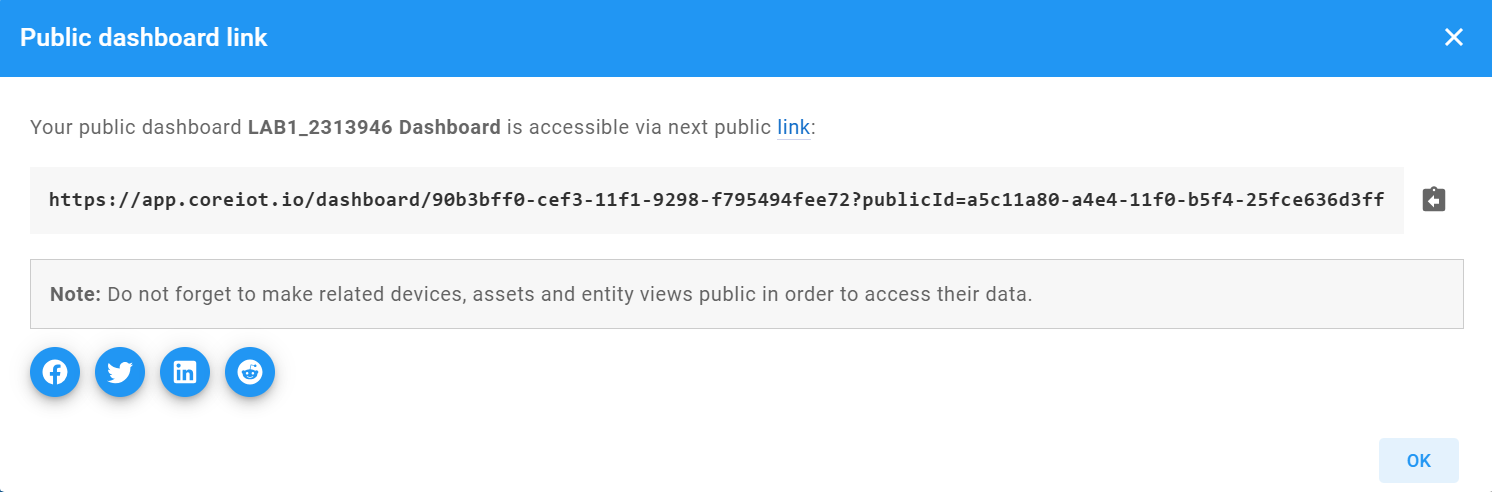
\includegraphics[width=0.92\textwidth]{image/anh5_1.png}
    \caption{Hộp thoại Public dashboard link hiển thị đường link chia sẻ công khai}
    \label{fig:anh5_1}
\end{figure}

\begin{figure}[H]
    \centering
    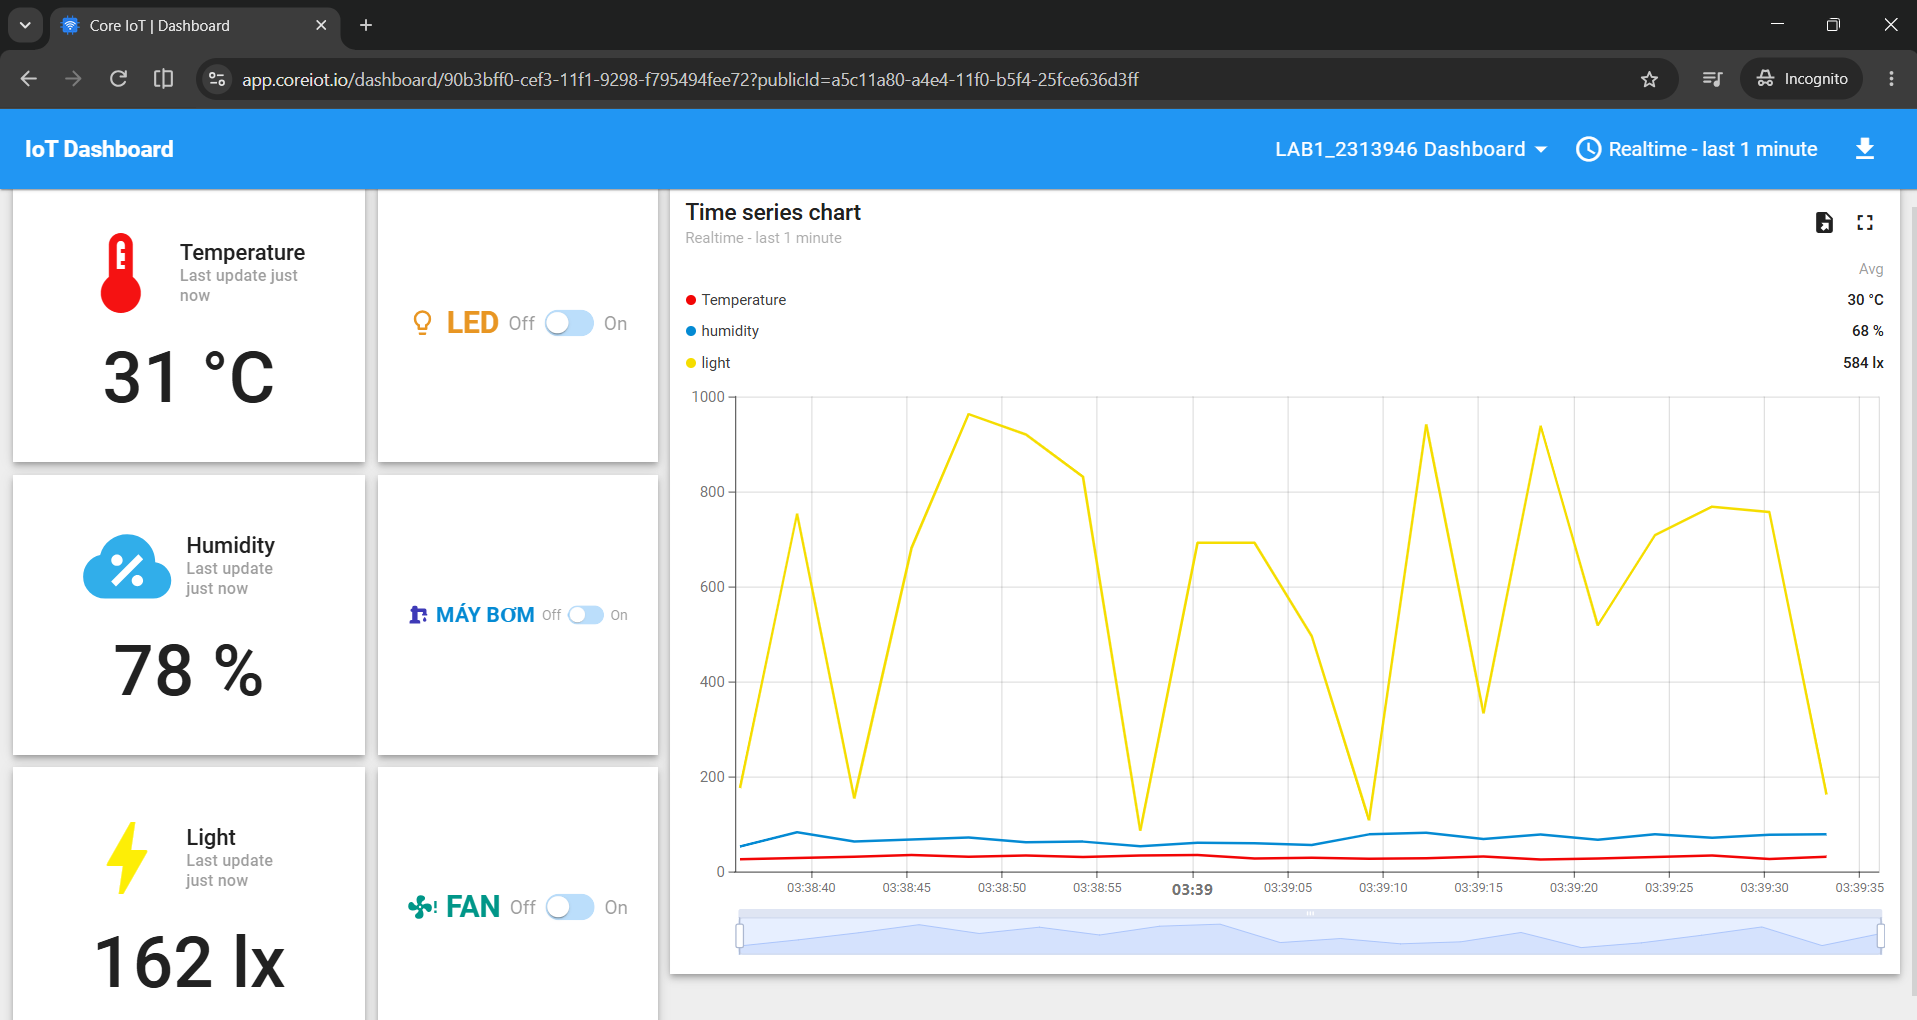
\includegraphics[width=0.95\textwidth]{image/anh5_2.png}
    \caption{Toàn màn hình Dashboard mở trên trình duyệt ẩn danh (Incognito) hiển thị dữ liệu trực tiếp}
    \label{fig:anh5_2}
\end{figure}

\subsubsection{Trả lời câu hỏi bài tập 5}
\begin{tcolorbox}[colback=blue!5,colframe=blue!75!black,title=\textbf{Câu hỏi 5: Vì sao nhóm thiết bị cũng phải ở chế độ công khai? Điều gì có thể xảy ra nếu bạn đặt mọi dashboard và thiết bị trong tài khoản của mình ở chế độ công khai?}]
\textbf{Trả lời:}
\begin{itemize}
    \item \textbf{Vì sao nhóm thiết bị cũng phải công khai:} Trên nền tảng CoreIOT/ThingsBoard, Dashboard chỉ là tầng giao diện hiển thị dữ liệu trực quan, trong khi quyền đọc/ghi dữ liệu viễn trắc thuộc quyền sở hữu của thực thể (Device Entity). Khi người dùng ẩn danh truy cập qua Public Link, nếu nhóm thiết bị vẫn ở chế độ riêng tư (Private) thì máy chủ sẽ từ chối cung cấp dữ liệu cảm biến cho phiên truy cập ẩn danh đó, khiến toàn bộ các thẻ giá trị và biểu đồ đều bị trắng dữ liệu (\textit{"No data"}).
    \item \textbf{Hậu quả nếu đặt mọi thứ ở chế độ công khai:}
    \begin{enumerate}
        \item \textit{Rò rỉ dữ liệu nhạy cảm:} Toàn bộ số liệu đo đạc nội bộ, quy trình sinh hoạt, định vị vị trí và nhật ký vận hành đều bị công khai cho bất kỳ ai trên không gian mạng.
        \item \textit{Mất an toàn điều khiển phần cứng:} Nếu trên các Dashboard công khai có chứa các widget điều khiển RPC (như công tắc Bơm, Đèn, Quạt, Relay), bất kỳ người lạ nào cũng có thể tự do bật/tắt thiết bị vật lý thật ngoài đời thực, dẫn đến nguy cơ xung đột vận hành, hỏng hóc máy móc hoặc gây ra các sự cố cháy nổ nguy hiểm.
    \end{enumerate}
\end{itemize}
\end{tcolorbox}
